\chapter{Analyse der Anwendung}\label{chapter_3}
Damit der Konfigurationsprozess für den Kunden einfacher wird, muss im ersten Schritt der aktuelle Prozess analysiert werden. Darauf aufbauend werden Konzepte zur Vereinfachung dieses Prozesses überlegt und ein neuer Workflow erstellt. Die Anforderungen an die neue Anwendung werden anschließend spezifiziert.

\section{Aktueller Konfigurationsprozess}
Die Anpassungen und Vereinfachung eines Konfigurationsprozesses bei der Verwendung von mobilen Anwendungen soll am konkreten Anwendungsbeispiel gezeigt werden. Die Analyse beginnt bei grundlegenden Fragen, wie ein solcher Prozess aufgebaut ist und wird im Folgenden anhand eines konkreten Kundenfall weiter ausgebaut.

\begin{figure}
\label{oldWorkflow}
\centering
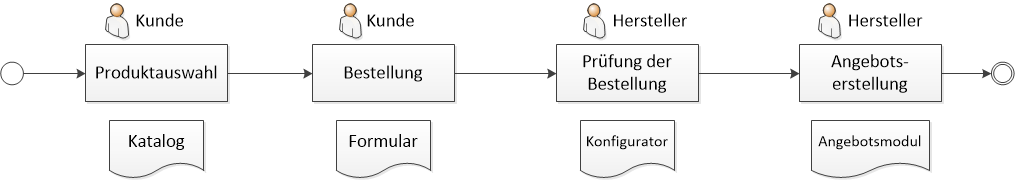
\includegraphics[width=\hsize]{images/konfigurationsprozess_alt}
\caption{Auszug eines Konfigurationsprozesses}
\end{figure}
Ein Auszug aus einem Konfigurationsprozess ist in Abbildung  \ref{oldWorkflow} zu sehen. Der Prozess beginnt mit der Produktauswahl. Zu Beginn möchte der Kunde ein konkretes Produkt auswählen. Dies geschieht über den Produktkatalog. In diesem findet er sein gewünschtes Produkt. Anschließend kann er mithilfe von eindeutigen Produktnummern die Bestellung über ein Formular weitergeben. Damit die Zusammenstellung des Kunden geprüft werden kann, werden die Daten beim Hersteller in das Konfigurationssystem eingepflegt. Dieses berechnet die komplexen Abhängigkeiten und prüft die Gültigkeit der Konfiguration. Der letzte Schritt ist die Angebotserstellung. Hierbei wird das konkrete Angebot für den Kunden erstellt.
\par

Bei der Verwendung dieser Prozessbeschreibung entstehen Probleme, die eine Vereinfachung des Prozesses erschweren. Erstes Problem ist die Verwendung von Produktnummern. Diese Nummern werden für eine eindeutige Identifizierung des Produktes bei der Bestellung verwendet. Bei der Verwendung können Fehler entstehen. Es kann die falsche Produktnummer vom Kunden bei der Auswahl verwendet werden, so dass nicht das richtige Produkt bei der Angebotserstellung verwendet wird. Bei der Produktauswahl sind 
diese Informationen nicht notwendig, da der Kunde sich nur für das konkrete Produkt interessiert. Für die Vereinfachung des Prozesses ist eine automatische Zuordnung der korrekten Nummer im Hintergrund die Lösung. Somit wird der direkte Umgang des Kunden mit einzelnen Produktnummern vermieden und die alleinige Auswahl des Produktes steht für den Kunden im Vordergrund. Hierdurch wird der Prozess vereinfacht. \par

Die zweite Stelle, an der eine Verbesserung möglich ist, befindet sich bei der Eingabe der Daten für den Produktkonfigurator und der damit verbundenen Prüfung. Der Kunde hat im vorigen Schritt bereits die Daten, die benötigt werden erfasst. Eine zweite Erfassung kann zu Fehlern oder Kommunikationsproblemen führen. Diese Probleme entstehen bei der falschen Eingabe des bestellten Produktes. Hierdurch kann der Konfigurator ein falsches Ergebnis liefern, welches zu einem inkorrekten Angebot führt, wodurch der Prozess wiederholt werden muss. Für die Verbesserung dieser Situation muss die Eingabe des Kunden direkt zum Konfigurator gegeben werden. Diese Maßnahme minimiert die Fehler bei der Erfassung. 

Weiterhin entsteht durch den gegebenen Prozess ein Kommunikationsproblem. Dies tritt aufgrund der Trennung von Produktauswahl und Produktkonfiguration auf. Der Kunde ist nur bei der Auswahl beteiligt. Das Feedback für die Umsetzung der Zusammenstellung erfolgt erst nach der Weitergabe der Bestellung. Dies ist problematisch, wenn bei der Konfiguration Alternativen auftreten, bei denen der Kunde entscheiden muss oder eine Konfiguration komplett nicht umsetzbar ist. Hier muss ggf. der Prozess wiederholt werden. Für die Lösung ist eine Hinzunahme des Kunden bei der Konfigurationsüberprüfung notwendig. Das Ziel sollte ein schnelles Feedback bei der aktuellen Auswahl sein. 

Zusammenfassend treten drei grundlegende Probleme bei einem Konfigurationsprozess auf:
\begin{itemize}
        \item Produktnummern sind für den Kunden schwierig zu handhaben.
        
        \item Daten werden doppelt erfasst.
        
        \item zusätzlicher Kommunikationsaufwand durch zu spätes Feedback
\end{itemize}
Diese drei Punkte werden in der Modellierung des neuen Workflows verbessert.

\subsection{Übertragung auf den Kunden}
Beim Anwendungsbeispiel des Kunden erfolgt die Auswahl der Upgrades ebenfalls über einen Produktkatalog. In diesem Katalog sind die einzelnen Upgrades aufgeführt. Die Auswahl der Produkte erfolgt über eine vorhandene Weboberfläche. Diese Oberfläche ist über die Homepage des Kunden verfügbar. Der Endkunde, im Anwendungsbeispiel eine Fluggesellschaft wählt das gewünschte Upgrade aus dem Katalog aus. Bei der Bestellung werden die Produktcodes der Auswahl verwendet. Zusätzlich müssen die Flugzeuge angegeben werden, die das Upgrade erhalten sollen. Die Identifizierung erfolgt ebenfalls anhand des eindeutigen Flugzeugcodes. Beide Codes werden im nächsten Schritt von einem Produktkonfigurator erfasst und anschließend eine Überprüfung der Konfiguration durchgeführt.   \par 

Beim Kunden wird die klare Trennung der Auswahl und der Überprüfung durch die Verwendung von zwei unterschiedlichen Systemen deutlich. Die Kommunikation der beiden Systeme erfolgt über die Produkt-, bzw. Flugzeugcodes. Bei der Überprüfung der Konfiguration ist der Kunde  nicht involviert. Der Experte bearbeitet die Bestellung und pflegt diese in das System ein. Bei der Umstellung des Prozesses muss auch dieser Vorgang der Konfiguration verstanden werden, um die Eignung für den neuen Workflow herauszufinden. \par 
\begin{figure}
\label{webguiAblauf}
\centering
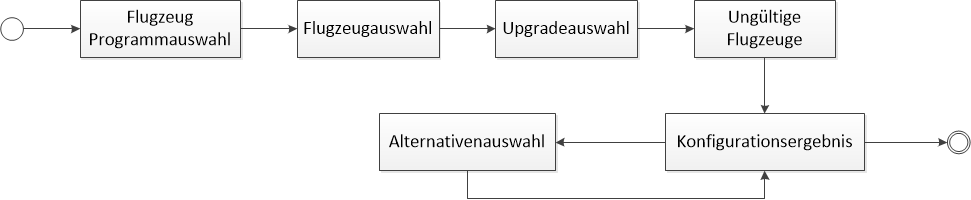
\includegraphics[width=300px]{images/workflow_webgui}
\caption{Programmablauf der Konfigurationslösung}
\end{figure}

Abbildung \ref{webguiAblauf} zeigt den Ablauf einer Konfiguration mit dem derzeitigen System.
Im ersten Schritt wird das passende Flugzeugprogramm ausgewählt. Ein Programm ist eine grobe Einteilung für Flugzeuge nach deren Größe und Art. Die Auswahl ist eine erste Filterung der Datensätze. Des weiteren werden mit Hilfe des Programms die Regeln ausgewählt, die auf dem Konfigurationsserver verwendet werden. Anschließend folgt die Auswahl der entsprechenden Flugzeuge, welche ein Upgrade erhalten sollen. Die Auswahl kann nach bestimmten Kriterien gefiltert werden. Bei der Bestellung eines Upgrades wird die Flugzeugnummer angegeben, womit eine schnelle Auswahl erfolgen kann. Sind die Flugzeuge ausgewählt, werden Upgrades aus einer Liste selektiert. Es sind alle verfügbaren Updates aufgelistet. Die Auswahl erfolgt ebenfalls mit der eindeutigen Nummer, welche bei der Bestellung angegeben wurde. \par 

Nach der letzten Auswahl sind alle für die Konfiguration benötigten Elemente ausgewählt. Es folgt eine Validierung der Flugzeuge. Bei dieser Überprüfung werden die einzelnen Flugzeuge auf Konfigurationen untersucht, die in Widerspruch mit dem ausgewählten Upgrade stehen. Wenn keine Widersprüche vorhanden sind, werden sogenannte Konfigurationsgruppen gebildet. Eine Konfigurationsgruppe enthält Flugzeuge, die in die gleichen Zielzustände kommen, wenn das Upgrade eingebaut wird. Wenn es mehrere Möglichkeiten gibt, um in einen bestimmten Zustand des Flugzeuges zu kommen, werden sogenannte Alternativen in einer Konfigurationsgruppe enthalten. Damit die Konfiguration vollständig ist, muss der Anwender für die Gruppe eine Alternative auswählen. \par

Nachdem eine vollständige Konfiguration erzeugt wurde, wird daraus ein Excel-Dokument generiert. In diesem sind die Upgrades enthalten, die in den einzelnen Flugzeuge eingebaut werden müssen. Aus dem Dokument wird ein Upgrade-Angebot erstellt, dass anschließend dem Kunden vorgelegt wird. \par 

Das Hauptproblem des aktuellen Systems ist, dass nur Experten die Anwendung bedienen können. Eine effektive Nutzung kann nur mithilfe der Produktcodes erfolgen. Dies führt dazu, dass man ein großes Wissen über die Produktstruktur besitzen muss. Dadurch kann mit der aktuellen Anwendung der Kunde die Konfiguration nicht selbstständig durchführen. Dieses Problem wird im Folgenden bei der Modellierung des neuen Workflows gelöst.

\section{Workflow Modellierung}
Der neue Workflow muss die im vorigen Abschnitt erwähnten Probleme des Konfigurationsprozesses lösen.  Anschließend müssen die Lösungen auf den konkreten Anwendungsfall übertragen werden und ein neuer Programmablauf gefunden werden, der den Lösungsweg beinhaltet.

\subsection{Mobiler Konfigurationsprozess}\label{mobileConfiguration}
Die Probleme mit der Verwendung von Produktnummern und die doppelte Erfassung der Daten lassen sich durch die Zusammenlegung von Auswahl und Konfigurationsprüfung mit einem System lösen. Dieses Zusammenlegen von Produktauswahl und Produktkonfiguration in einer Anwendung ermöglicht es dem Kunden die gewünschte Auswahl zu tätigen und gleichzeitig ein Feedback der Konfiguration zu erhalten. Durch die bessere Rückmeldung verringert sich der Kommunikationsaufwand, da der Kunde im Idealfalls sofort das Resultat sieht. \par 
 Für eine noch bessere Unterstützung, sowie Hilfestellung beim Aufkommen von Alternativen ist die Durchführung des Prozesses mit einem Mitarbeiter des Herstellers von Vorteil. Dieser kann den Kunden durch die Konfiguration führen oder unterstützen. Gleichzeitig wird hier ein besseres Verständnis für das Produkt ermöglicht. Der Herstelle hat den Vorteil der Beschleunigung des Prozesses. Er kann durch die direkte Auswahl der Produkte, sowie ein sofortiges Prüfen und ggf. eine Selektion der Alternativen die Konfiguration abschließen und ein konkretes Angebot erstellen. \par 
 
Diese Umstellungen des Prozesses setzt die Verwendung eines mobilen Endgerätes, in diesem Fall einem Tablet-PC voraus. Durch die Mobilität des Gerätes kann die Konfiguration direkt beim Kunden vor Ort durchgeführt werden. Die verbesserte Kommunikationsmöglichkeit mithilfe des Tablets sorgt für ein besseres Verständnis des Kunden und dessen Wünsche. 


Zusammenfassend sind folgende zwei Maßnahmen beim neuen Workflow durchzuführen: \par

\begin{itemize}
        \item Zusammenlegen von Produktauswahl und Produktkonfiguration. 
        \item Unterstützung durch einen Mitarbeiter des Herstellers.
\end{itemize}
Die konkrete Umsetzung dieser beiden Änderungen wird im Folgenden am Anwendungsbeispiel durchgeführt. \par

\subsection{Workflow des Anwendungsbeispiels}
Für die Umsetzung der aus Abschnitt \ref{mobileConfiguration} erstellten Maßnahmen müssen die beiden vorhandenen Systeme für die Auswahl und Konfiguration auf ein gemeinsames Gerät portiert werden. Das Konfigurationssystem muss hierfür vereinfacht werden, um den Zugang für den Kunden zu erleichtern. Die Herausforderung besteht hier in einer übersichtlichen Darstellung der Konfigurationsergebnisse. Diese müssen für den Kunden nachvollziehbar aufbereitet werden, da er nicht die Produktkenntnisse des Experten besitzt. Da der Kunde die Auswahl der einzelnen Produkte "'live"' vornimmt, muss die Anwendung ein schnelleres Feedback erzeugen. Bei der vorherigen Lösung hat der Experte die komplette Zusammenstellung des Kunden erhalten und musste diese in das System übertragen. Beim neuen Workflow dagegen möchte der Kunde die Reihenfolge bei der Auswahl selbst bestimmen. Dies muss im neuen Anwendungsverlauf berücksichtigt werden. \par 
\begin{figure}
\label{appWorkflow}
\centering
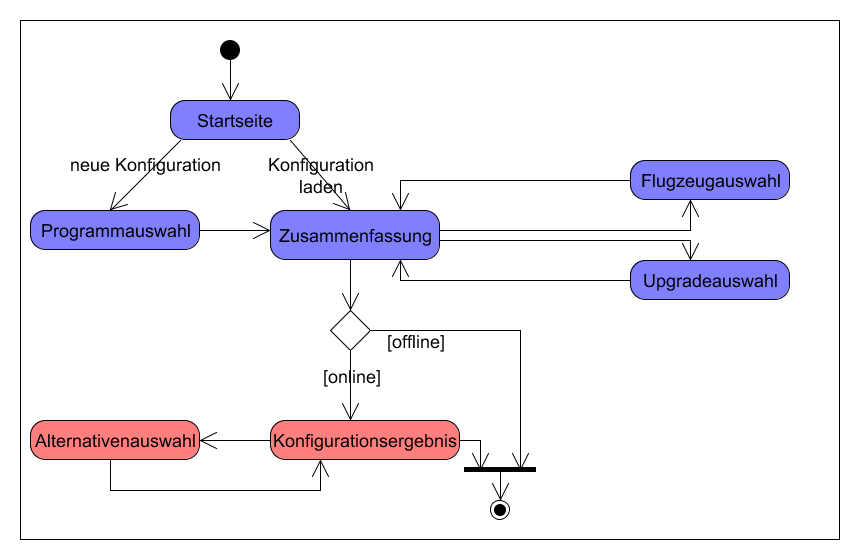
\includegraphics[width=400px]{images/workflow_app}
\caption{Programmablauf der Konfigurator-App}
\end{figure}
In Abbildung \ref{appWorkflow} ist der Anwendungsverlauf der App zu sehen. Analog zu der Weboberfläche wird bei einer neuen Konfiguration zuerst ein Programm (\textbf{Programmauswahl}) ausgewählt. Dies ist aufgrund einer Filterung der Daten weiterhin notwendig. Nach der Auswahl gelangt der Benutzer in eine \textbf{Zusammenfassung} der aktuellen Konfiguration. Von dieser Ansicht aus können Flugzeuge (\textbf{Flugzeugauswahl}) oder  Upgrades (\textbf{Upgradeauswahl}) selektiert werden. Hier wird den unterschiedlichen Bedürfnissen des Kunden entsprochen und kein strikter Konfigurationsablauf vorgegeben, wie es im vorherigen System war. Mit dieser Umstellung wird dem Kunden die Möglichkeit gegeben die einzelnen Upgrades nacheinander zu wählen und jederzeit eine schnelle Änderung zu ermöglichen. Sobald mindestens ein Flugzeug oder ein Upgrade ausgewählt ist, wird die Konfiguration überprüft. 
Nach der Überprüfung werden die  Konfigurationsgruppen, die der Konfigurator erstellt hat angezeigt. Diese Gruppen kann der Benutzer einsehen und bei mehreren Alternativen in einer 
separaten Ansicht (\textbf{Alternativenauswahl}) die richtige Lösung auswählen. Ist die Konfiguration vollständig, so hat der Nutzer die Möglichkeit die aktuelle Zusammenstellung zu bestellen und den Vorgang mit der Bestellung zu beenden. 

Da die Verwendung des Konfigurationsservers, wie in Kapitel \ref{configurator} beschrieben nach dem Client-Server Modell aufgebaut ist, wird eine andere Möglichkeit bei der Konfiguration nötig. Beim mobilen Einsatz der Anwendung kann es passieren, dass eine Verbindung mit dem Konfigurationsserver nicht möglich ist. Aus diesem Grund muss es einen alternativen Weg des Workflows geben. Wenn der Konfigurationsserver nicht verfügbar ist, wird die Konfiguration gespeichert, damit eine Prüfung später durchgeführt werden kann. In diesem Fall ist der Prozesses mit der Speicherung der Konfiguration beendet.


\section{Anforderungsanalyse} \label{requirements}
Nachdem der grundlegende Prozess auf die Bedürfnisse des Kunden, sowie an die mobile Umgebung angepasst sind, können daraus die Anforderungen der Anwendung für das Anwendungsbeispiel festgelegt werden. Bei der Festlegung wird zuerst die allgemeine Anforderung erläutert, sowie anschließend auf das Anwendungsbeispiel spezifiziert. Für eine einfachere Darstellung wird im Folgenden zwischen Funktionalen und Nicht-Funktionalen Anforderungen unterschieden. 

\subsection{Nicht-Funktionale Anforderungen}\label{non_functional_requirements}
Die Nicht-Funktionalen Anforderungen betreffen alle Maßnahmen zur Vereinfachung, bzw. Unterstützung des Prozesses, sowie Anforderungen aufgrund des vorhandenen Systems. Diese speziellen Voraussetzungen sind für den Benutzer meistens nicht sichtbar und laufen im Hintergrund, bzw. Unbewusst ab. Aus diesem Grund müssen hier auch spezielle Gütekriterien festgelegt werden, um am Ende eine Evaluation zu ermöglichen. Für den neuen Workflow wurden folgende Anforderungen spezifiziert:


\paragraph{Einfache Bedienung:} Dadurch, dass der Kunde kein Experte ist und die Anwendung nicht jeden Tag verwendet, muss die Bedienung für den Kunden einfach sein. Je weniger bei der Verwendung der Software erklärt werden muss, desto besser ist diese Anforderung erfüllt. Für die Erfüllung dieses Ziels sollen Folgende Schwerpunkte der Softwareergonomie behandelt werden: 
\begin{itemize}
        \item Selbstbeschreibungsfähigkeit
        \item Lernförderlichkeit
        \item Erwartungskonformität
     \end{itemize}


\begin{tabular}[H]{| p{0.5cm} | p{2.2cm} | p{4.5cm} | p{5.3cm} | p{1.3cm} |}
\toprule[2pt] \rowcolor{dunkelgrau}
\hline
  NR. & Anforderung & Beschreibung & Details & Priorität \\
  \hline
  N1 & Einfache \newline Bedienung & Die Anwendung soll von unerfahrenen Benutzern schnell bedient werden können.& Schwerpunkte der Softwareergonomie\cite{bib:softwareErgonomie}: 
  \begin{itemize}
        \item Selbstbeschreibungs-fähigkeit
        \item Lernförderlichkeit
        \item Erwartungs-konformität
     \end{itemize}
   & A \\
  \hline
  N2 & Schnelle Bedienung & Die Auswahl der einzelnen Komponenten soll möglichst schnell getätigt werden können. & Es muss für eine flüssige Navigation zwischen den einzelnen Seiten gesorgt werden. Der Benutzer sollte keine langen Wartezeiten beim Bedienen der Anwendung haben. & A \\
  \hline
    N3 & Offline-Online Modus & Die Anwendung soll einen Offline- und Online-Modus enthalten & Es sollen Konfigurationsdaten offline zusammengestellt werden können, die später oder zeitgleich online (mit Konfigurationsserver) geprüft werden. & A \\
    \hline
    N4 & Allein-stellungs-merkmal & Um den Kunden zu begeistern ist ein besonderes Feature, welches die Anwendung als Alleinstellungsmerkmal besitzt wünschenswert.& Es sollen besonders "'aufregende"' Features, die eine Technologie bietet in die Anwendung integriert und in einem sinnvollen Kontext genutzt werden.  & B\\
    \hline
\bottomrule[2pt]
\end{tabular}

\subsection{Funktionale Anforderungen}
Eine funktionale Anforderung betrifft den Prozess, bspw. die Auswahl eines Upgrades.
\begin{tabular}[H]{| p{0.4cm} | p{2.3cm} | p{4.5cm} | p{5.3cm} | p{1.3cm} |}
\toprule[2pt] \rowcolor{dunkelgrau}
\hline
  NR. & Anforderung & Beschreibung & Details & Priorität \\
  \hline
  F1 & Upgrade-auswahl & Es sollen Upgrades für Flugzeuge auswählbar sein & Bevor die Auswahl stattfindet, soll es verschiedene Filtermöglichkeiten geben, wie beispielsweise der Flugzeugtyp oder die Art des Upgrades.
   & A \\
  \hline
  F2 & Flugzeug-auswahl & Es müssen Flugzeuge eines bestimmten Kunden auswählbar sein. & Es soll auch hier, analog zu B1 die Möglichkeit der Auswahl von Flugzeugen auf einen vorher gefilterten Datensatz geben. & A \\
  \hline
    F3 & Konfiguration & Nach erfolgter Auswahl werden die Ergebnisse der Konfiguration dargestellt. & Kommunikation mit dem Konfigurationsserver, sowie die Darstellung der Ergebnisse auf dem Client& A \\
    \hline
     F4 & Alternativen & Bei mehreren Möglichkeiten einer Auswahl sollen Alternativen ausgewählt werden können & Übersichtliche Darstellung von Alternativenauswahl.& A \\
        \hline
    F5 & Speichern & Die getätigte Auswahl soll gespeichert werden& Nach Abschluss der Konfiguration soll diese lokal gespeichert werden, um ein erneutes Laden zu ermöglichen. & B\\
    \hline
    F6 & Laden & Getätigte Konfigurationen müssen geladen werden können& Beim Start der Anwendung sollen getätigte Konfigurationen geladen und angezeigt werden können & B\\
    \hline
\bottomrule[2pt]
\end{tabular}





